%\documentclass[overheadsbeamer.tex]{subfiles}
\documentclass[handoutsbeamer.tex]{subfiles}

\begin{document}

\thispagestyle{empty}

\ona{ \setcounter{chapter}{0} } % ONE LESS
\lecture{Two Perspectives on Variational Methods: Molecules and Cuts}{Lect01}
\chapter{Two Perspectives on Variational Methods: Molecules and Cuts}\label{C.Motivation}

\section{The plan of the course}

\begin{frame}\ft{Roadmap}
\ona{The course is organised around one algorithmic idea, the variational method, seen from two sides, physical chemistry and theoretical computer science, and around the three questions one should ask of any heuristic: does it converge, how fast, and how good is the answer. The thirteen lectures are:}
\onp{\footnotesize}
\begin{enumerate}\setlength\itemsep{0.05em}
    \item Two perspectives: molecular energy levels versus MaxCut (today, \Chap~\chref{C.Motivation}).
    \item The exponential quantum advantage hypothesis (\Chap~\chref{C.EQA}).
    \item Inapproximability and the Unique Games Conjecture (\Chap~\chref{C.Inapprox}).
    \item The adiabatic theorem and quantum speedup via quantum annealing (\Chap~\chref{C.Annealing}).
    \item The variational quantum eigensolver (\Chap~\chref{C.VQE}).
    \item The quantum approximate optimization algorithm, and its convergence (\Chap~\chref{C.QAOA}).
    \item The parameter-shift rule (\Chap~\chref{C.PSR}).
    \item Iteration complexity of QAOA with the parameter-shift rule (\Chap~\chref{C.IterationComplexity}).
    \item Per-iteration complexity of QAOA (\Chap~\chref{C.PerIteration}).
    \item Warm-started quantum optimization: rounded (\Chap~\chref{C.WSRounded}).
    \item Warm-started quantum optimization: continuous (\Chap~\chref{C.WSContinuous}).
    \item Applications: variational solvers for systems of linear equations (\Chap~\chref{C.VQLS}).
    \item Applications: variational solvers for Markowitz portfolio management (\Chap~\chref{C.Portfolio}).
\end{enumerate}
\end{frame}

\begin{frame}\ft{Course organisation: the team}
% Organisation copied from organization.tex (the quantum optimal control course), as requested.
\begin{itemize}\setlength\itemsep{0.3em}
    \item \textbf{Jakub Mare{\v c}ek} lectures\ona{ and is responsible for the course}. \\ {\small\texttt{jakub.marecek@fel.cvut.cz}}
    \item \textbf{Ruben Karapetyan} is the teaching assistant\ona{ and leads the practical classes}. \\ {\small\texttt{karaprub@fjfi.cvut.cz}}
\end{itemize}
\medskip
\textbf{Lectures/Tutorials:} Thursdays, 9:15--10:45 and 11:00--12:30, room KN:A-224.
\medskip

\textbf{Materials:} slides and handouts share one source; the lecture notes are self-contained, and each \chap{} is based on one paper, which is cited at its start.
\end{frame}

\begin{frame}\ft{Prerequisites}
\textbf{There are no formal prerequisites.}

\ona{We assume linear algebra (eigenvalues and eigenvectors of Hermitian matrices, tensor products) and basic probability. No prior knowledge of quantum mechanics is assumed: \Chap~\chref{C.VQE} summarises what is needed, namely that a state of $n$ qubits is a unit vector in $\C^{2^n}$, that an observable is a Hermitian matrix, and that its expectation in a state is a Rayleigh quotient. No prior knowledge of optimization beyond calculus is assumed either; convex relaxations and semidefinite programming are introduced in \Chap~\chref{C.WSRounded} when they are needed.}
\onp{\begin{itemize}
    \item Useful background: linear algebra (spectral theorem, tensor products), basic probability. \emph{No} quantum mechanics assumed; \Chap~\chref{C.VQE} recaps what is needed.
    \item Useful background in optimization: gradient descent and convex relaxations; both are introduced when needed.
    \item Optional reading: \citet{kristaly2010variational}, \emph{Variational Principles in Mathematical Physics, Geometry, and Economics}; the survey \cite{abbas2024challenges}; and the papers the individual lectures are based on.
\end{itemize}}
\ona{Optional reading material: for the mathematics of variational principles in general, \citet{kristaly2010variational}, \emph{Variational Principles in Mathematical Physics, Geometry, and Economics}, Encyclopedia of Mathematics and its Applications 136, Cambridge University Press, 2010; for quantum optimization, the survey of \citet{abbas2024challenges}, \emph{Challenges and Opportunities in Quantum Optimization}, from which \Chaps~\chref{C.EQA}--\chref{C.Inapprox} draw. None of it is required.}
\end{frame}

\begin{frame}\ft{Assessment}
In total, you can earn a maximum of 100 points for the course and receive a grade from A to F ($<50$ points $=$ F, 50--59 $=$ E, 60--69 $=$ D, 70--79 $=$ C, 80--89 $=$ B, 90--100 $=$ A).
Points are earned through semester activities (up to 60 points in total) and the exam (up to 40 points).

\textbf{Course credit: semester activity (max.\ 60 points).}
You can earn semester points by completing assignments.
For all assignments, the last submitted solution is the one considered for grading.
To receive course credit, you must earn at least 30 out of 60 points and attend the practical classes regularly. One absence is permitted.

\textbf{Exam (max.\ 40 points).}
Theoretical part of the exam (max.\ 40 points)\ona{, covering \Chaps~\chref{C.EQA}--\chref{C.Portfolio}}. If multiple successful attempts are made, the highest score achieved is considered.
\end{frame}

\section{Two perspectives at a glance}

\begin{frame}\ft{Two communities, one object}
\onp{\scriptsize}
\ona{Physical chemists and theoretical computer scientists study the same mathematical object, a Hermitian matrix and its lowest eigenvector, with different vocabularies, different yardsticks, and different classical competitors. This lecture introduces both, and the rest of the course moves between them.}
\begin{center}\ona{\small}
\begin{tabular}{lll}\toprule
 & physical chemistry & theoretical computer science \\\midrule
Hamiltonian $H$ & molecular, $\mathcal O(M^4)$ Pauli terms & diagonal Ising, $|E|$ terms \\
ground state & correlated electronic state & a bitstring, the optimal cut \\
$E_0$ & ground-state energy & optimal value $\mathrm{OPT}$ \\
quality & error in Hartree & approximation ratio \\
competitor & coupled cluster, DMRG & GW, local search \\
overlap $\eta$ & of Hartree--Fock with $\ket{\psi_0}$ & $\mathrm{Pr}[\text{sample is optimal}]$ \\
hardness & $\mathbf{QMA}$-hard in general & $\mathbf{NP}$-hard; $\mathbf{APX}$-hard \\\bottomrule
\end{tabular}
\end{center}
\onp{\medskip Same object, two vocabularies; the course moves between them.}
\end{frame}

\section{Perspective one: physical chemistry}

\begin{frame}\ft{Why molecules?}
\ona{Simulating molecules and materials is the application for which quantum computers were first proposed, and it remains the one with the clearest physical motivation: the objects are themselves quantum mechanical.}
\begin{itemize}\setlength\itemsep{0.3em}
    \item \textbf{What is computed:} energies of molecules and materials, and from them reaction rates, binding affinities in drug design, catalytic pathways (nitrogen fixation by the FeMo cofactor of nitrogenase is the standard example), band structures, and spectra.
    \item \textbf{Why it is hard:} the wave function of $N$ electrons in $M$ orbitals lives in a space of dimension $\binom{M}{N}$; exact treatment is exponential, and a large share of the world's supercomputing time goes into approximating it.
    \item \textbf{Why quantum computers:} $M$ qubits hold the wave function natively; phase estimation was proposed for molecular energies in 2005, and the variational quantum eigensolver of \citet{peruzzo2014variational} was the first algorithm run on hardware for this purpose.
    \item \textbf{What is at stake:} chemical accuracy, $1.6\times10^{-3}$ Hartree ($1$ kcal/mol), the precision at which reaction rates at room temperature are predicted to within an order of magnitude.
\end{itemize}
\end{frame}

\begin{frame}\ft{The smallest molecule}
\ona{Molecular hydrogen, H$_2$: two protons at distance $R$ ($R_{\rm eq} \approx 0.74$ \AA{} $= 1.40$ Bohr) and two electrons. Figure~\ref{fig:ch01:h2mol} shows the nuclei and the electron density of the bonding state, concentrated between the nuclei.}
\begin{center}
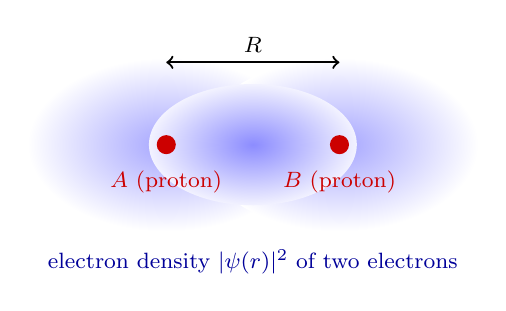
\begin{tikzpicture}[scale=1.1]
  % electron cloud: overlapping shaded blobs
  \shade[inner color=blue!35, outer color=white] (-1.0,0) ellipse (1.6 and 1.0);
  \shade[inner color=blue!35, outer color=white] ( 1.0,0) ellipse (1.6 and 1.0);
  \shade[inner color=blue!45, outer color=blue!5] (0,0) ellipse (1.2 and 0.7);
  % nuclei
  \fill[red!80!black] (-1,0) circle (0.11) node[below=6pt] {\footnotesize $A$ (proton)};
  \fill[red!80!black] ( 1,0) circle (0.11) node[below=6pt] {\footnotesize $B$ (proton)};
  \draw[<->,thick] (-1,0.95) -- (1,0.95) node[midway,above] {\footnotesize $R$};
  \node[blue!60!black] at (0,-1.35) {\footnotesize electron density $|\psi(\boldsymbol r)|^2$ of two electrons};
\end{tikzpicture}
\end{center}
\ona{\begin{figure}[htb]\caption{Schematic of H$_2$: two protons at distance $R$ and the electron density of the bonding ground state.}\label{fig:ch01:h2mol}\end{figure}}
\ona{Everything that follows in this course, including the QAOA circuits of hundreds of qubits, descends from the question of how to compute the energy of this system as a function of $R$.}
\end{frame}

\begin{frame}\ft{The Hamiltonian, specialised to H$_2$}
\ona{With the nuclei fixed (Born--Oppenheimer), the electronic Hamiltonian in atomic units is}
\begin{equation}\label{eq:ch01:h2first}
    H = -\tfrac12\nabla_1^2 - \tfrac12\nabla_2^2 - \sum_{i=1}^2\Big(\frac{1}{|\boldsymbol r_i - \boldsymbol R_A|} + \frac{1}{|\boldsymbol r_i - \boldsymbol R_B|}\Big) + \frac{1}{|\boldsymbol r_1 - \boldsymbol r_2|} + \frac1R,
\end{equation}
\ona{kinetic energy, attraction to the two nuclei, electron repulsion, nuclear repulsion. In the minimal basis (one $1s$ orbital per atom, STO-3G) there are two spatial orbitals, the bonding $\sigma_g$ and antibonding $\sigma_u$ combinations, hence four spin-orbitals and four qubits; using spin and parity symmetries, the two-electron problem reduces to two qubits and the Hamiltonian to six Pauli terms \cite{omalley2016scalable},}
\begin{equation}\label{eq:ch01:h2qubit}
    H = g_0\,\one + g_1 Z_0 + g_2 Z_1 + g_3 Z_0Z_1 + g_4 X_0X_1 + g_5 Y_0Y_1,
\end{equation}
\ona{with coefficients $g_k(R)$ computed classically from the one- and two-electron integrals. At $R = 0.75$ \AA: $g_0 = -0.4804$, $g_1 = 0.3435$, $g_2 = -0.4347$, $g_3 = 0.5716$, $g_4 = g_5 = 0.0910$ Hartree (electronic part; the nuclear repulsion $1/R$ is added separately).}
\onp{Minimal basis: two orbitals $\sigma_g,\sigma_u$ $\to$ four spin-orbitals $\to$ four qubits $\to$ two qubits by symmetry, six Pauli terms \cite{omalley2016scalable}; $g_k(R)$ from classical integrals.}
\end{frame}

\begin{frame}\ft{The wave function of H$_2$}
\ona{In the minimal basis the molecular orbitals are the symmetric and antisymmetric combinations of the atomic $1s$ orbitals $\phi_{A,B}(\boldsymbol r) \propto e^{-|\boldsymbol r - \boldsymbol R_{A,B}|}$, shown along the bond axis in Fig.~\ref{fig:ch01:h2wf}. Hartree--Fock puts both electrons (spin up and down) into $\sigma_g$: in the two-qubit encoding of \eqref{eq:ch01:h2qubit} this is the basis state $\ket{10}$, of energy $-1.83$ Hartree (electronic). The exact ground state mixes in the doubly excited configuration $\ket{01}$,}
\begin{equation}\label{eq:ch01:h2gs}
    \ket{\psi_0} = \cos\tfrac\theta2\,\ket{10} - \sin\tfrac\theta2\,\ket{01},\qquad \theta \approx 0.23 \text{ at } R = R_{\rm eq},
\end{equation}
\ona{which is exactly the one-parameter unitary coupled-cluster ansatz $e^{-i\theta/2\,(X_0Y_1 - Y_0X_1)/2}\ket{10}$: a variational circuit with a single angle, and the first VQE ever run on hardware \cite{omalley2016scalable}. The mixing grows with $R$ and becomes $\theta \to \pi/2$ at dissociation, where Hartree--Fock fails.}
\begin{center}
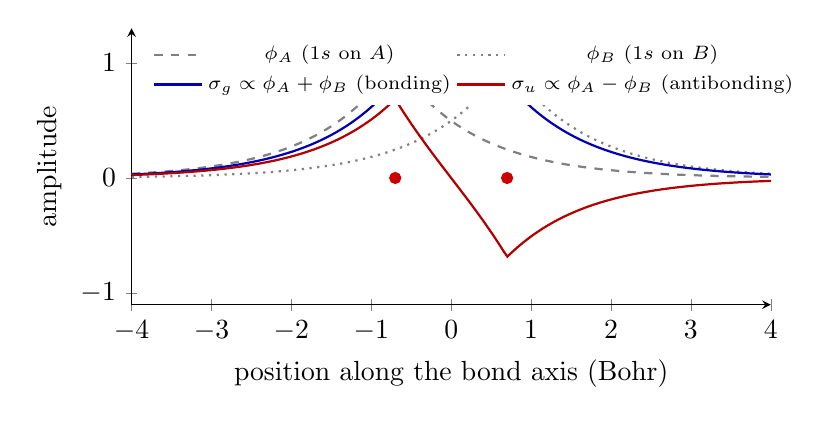
\begin{tikzpicture}
\begin{axis}[width=0.8\linewidth,height=0.42\linewidth,xlabel={position along the bond axis (Bohr)},ylabel={amplitude},xmin=-4,xmax=4,ymin=-1.1,ymax=1.3,axis lines=left,legend style={font=\scriptsize,draw=none,at={(0.02,0.98)},anchor=north west},legend columns=2,samples=200,domain=-4:4,no markers,every axis plot/.append style={thick}]
\addplot[gray,dashed] {exp(-abs(x+0.7))};
\addplot[gray,dotted] {exp(-abs(x-0.7))};
\addplot[blue!70!black] {(exp(-abs(x+0.7))+exp(-abs(x-0.7)))/1.5};
\addplot[red!70!black] {(exp(-abs(x+0.7))-exp(-abs(x-0.7)))/1.1};
\legend{$\phi_A$ ($1s$ on $A$),$\phi_B$ ($1s$ on $B$),$\sigma_g \propto \phi_A+\phi_B$ (bonding),$\sigma_u \propto \phi_A-\phi_B$ (antibonding)}
\draw[red!80!black,fill] (axis cs:-0.7,0) circle (2pt); \draw[red!80!black,fill] (axis cs:0.7,0) circle (2pt);
\end{axis}
\end{tikzpicture}
\end{center}
\ona{\begin{figure}[htb]\caption{Atomic $1s$ orbitals on the two protons (dots) and their bonding and antibonding combinations along the bond axis of H$_2$, minimal basis, schematic amplitudes.}\label{fig:ch01:h2wf}\end{figure}}
\end{frame}

\begin{frame}\ft{The energy levels of H$_2$}
\ona{Diagonalising the two-qubit Hamiltonian \eqref{eq:ch01:h2qubit} at $R = 0.75$ \AA{} gives four electronic energy levels, Fig.~\ref{fig:ch01:h2levels}. The ground state is the correlated singlet \eqref{eq:ch01:h2gs}; Hartree--Fock, the state $\ket{10}$, lies $0.02$ Hartree above it, about ten times chemical accuracy: this correlation energy is what the variational circuit must recover. The remaining levels are the excited configurations. Adding the nuclear repulsion $1/R \approx 0.706$ Hartree gives the total energies; repeating the calculation for every $R$ gives the potential-energy curves whose minimum is the bond length and whose curvature is the vibrational frequency.}
\begin{center}
\begin{tikzpicture}[x=1cm,y=1.9cm,every node/.style={font=\scriptsize}]
\draw[->] (0,-2.0) -- (0,0.35) node[above] {$E$ (Hartree, electronic)};
\foreach \y in {-2.0,-1.5,-1.0,-0.5,0} {\draw (-0.08,\y) -- (0.08,\y) node[left=6pt] {\y};}
\draw[very thick,blue!70!black] (1,-1.8512) -- (3.2,-1.8512) node[right,yshift=-4pt] {$E_0 = -1.851$: singlet ground state $\cos\tfrac\theta2\ket{10}-\sin\tfrac\theta2\ket{01}$};
\draw[thick,dashed,gray] (1,-1.8302) -- (3.2,-1.8302) node[right,gray,yshift=5pt] {Hartree--Fock $\ket{10}$: $-1.830$};
\draw[very thick,red!70!black] (1,-0.2528) -- (3.2,-0.2528) node[right] {$E_1 = -0.253$};
\draw[very thick,red!70!black] (1,0.0) -- (3.2,0.0) node[right] {$E_2 = 0.000$: triplet-like $\ket{00},\ket{11}$ sector};
\draw[very thick,red!70!black] (1,0.1824) -- (3.2,0.1824) node[right] {$E_3 = 0.182$: doubly excited};
\draw[<->,thick] (3.6,-1.8512) -- (3.6,-0.2528) node[midway,right] {gap $\gamma \approx 1.6$};
\end{tikzpicture}
\end{center}
\ona{\begin{figure}[htb]\caption{Electronic energy levels of H$_2$ in the minimal basis from the two-qubit Hamiltonian \eqref{eq:ch01:h2qubit} at $R = 0.75$ \AA{} (nuclear repulsion $1/R \approx 0.706$ Hartree not included). The dashed line is the Hartree--Fock energy; the difference to $E_0$ is the correlation energy.}\label{fig:ch01:h2levels}\end{figure}}
\ona{Three things to retain for the rest of the course: the ground state is what we want; a cheap trial state (Hartree--Fock) is close to it in energy and has large overlap with it, $|\braket{10|\psi_0}|^2 = \cos^2(\theta/2) \approx 0.99$; and there is a spectral gap $\gamma$ to the next level. Overlap and gap are exactly the two quantities on which the guarantees of the following slides, and of \Chap~\chref{C.EQA}, depend.}
\end{frame}


\begin{frame}\ft{Molecular energy levels}
\ona{Quantum computing for chemistry begins with a molecule: nuclei at fixed positions (Born--Oppenheimer) and $N$ electrons in a basis of $M$ spin-orbitals. In second quantisation the electronic Hamiltonian is}
\begin{equation}\label{eq:ch01:molH}
    H = \sum_{p,q} h_{pq}\,a_p^\dagger a_q + \frac12\sum_{p,q,r,s} h_{pqrs}\,a_p^\dagger a_q^\dagger a_r a_s,
\end{equation}
\ona{with one- and two-electron integrals $h_{pq}, h_{pqrs}$ computed classically, and after a Jordan--Wigner or Bravyi--Kitaev encoding it becomes a sum of $\mathcal O(M^4)$ Pauli strings on $M$ qubits. Its eigenvalues are the \emph{energy levels}; the lowest, $E_0$, is the ground-state energy, and differences of energy levels are what spectroscopy measures and what reaction rates depend on. Chemical accuracy is $1.6\times10^{-3}$ Hartree.}
\begin{itemize}\setlength\itemsep{0.2em}
    \item Exact diagonalisation (full configuration interaction) is exponential in $M$; classical heuristics (coupled cluster, DMRG, quantum Monte Carlo) are excellent for many molecules and fail for some strongly correlated ones.
    \item Quantum phase estimation returns $E_0$ to precision $\epsilon$ given a trial state with overlap $\eta = |\braket{\phi_0|\psi_0}|^2$ with the ground state, at cost $\widetilde{\mathcal O}(1/(\eta\epsilon))$ in evolution time, but needs deep, fault-tolerant circuits.
    \item The \emph{variational principle} is the classical chemist's tool for upper bounds on $E_0$; the variational quantum eigensolver (\Chap~\chref{C.VQE}) is its quantum-circuit version, and the origin of the word ``variational'' in this course.
\end{itemize}
\end{frame}

\begin{frame}\ft{Beyond the energy: ground-state properties}
\ona{For applications one needs more than $E_0$: dipole moments, charge densities, Green's functions, forces, i.e., expectations $\braket{\psi_0|O|\psi_0}$ of observables in the ground state. \citet{zhang2022computing} formalise this as the \emph{ground-state property estimation} problem: given $H$ with spectral gap $\gamma$, an observable $O$, a circuit preparing $\ket{\phi_0}$ with $|\braket{\phi_0|\psi_0}|^2 \ge \eta$, and $\epsilon$, estimate $\braket{\psi_0|O|\psi_0}$ to error $\epsilon$. Without the overlap and gap assumptions the decision version is $\mathsf{P^{QMA[\log]}}$-complete, harder than estimating the energy.}
\begin{itemize}\setlength\itemsep{0.2em}
    \item \textbf{Variational route:} run VQE to prepare an approximate ground state, then measure $O$. Cheap circuits, but no guarantee on the quality of the state, so no guarantee on the property.
    \item \textbf{Early fault-tolerant route} \cite{zhang2022computing}: use $\ket{\phi_0}$ only as a starting point with overlap $\eta$, and extract $\braket{\psi_0|O|\psi_0}$ from Hadamard tests of $e^{-ijH}$ and $O$ with classical Fourier post-processing. Maximal evolution time $\widetilde{\mathcal O}(\gamma^{-1})$, independent of $\epsilon$; total evolution time $\widetilde{\mathcal O}(\gamma^{-1}\epsilon^{-2}\eta^{-2})$; one ancilla qubit. Guaranteed accuracy \emph{regardless} of the quality of the variational state, at the price of runtime.
\end{itemize}
\ona{The two routes are complementary, and the variational one supplies the initial state for the other: this is the role we will assign to variational methods in chemistry in \Chaps~\chref{C.EQA} and~\chref{C.VQE}.}
\end{frame}

\begin{frame}\ft{How the guarantee works, in one slide}
\ona{Expand $\ket{\phi_0} = \sum_k\alpha_k\ket{\psi_k}$ in the eigenbasis of $H$, $p_k = |\alpha_k|^2$. The spectral measure $p(x) = \sum_kp_k\delta(x - \lambda_k)$ has cumulative distribution $C(x) = \sum_{\lambda_k\le x}p_k$, a step function whose first jump is at $\lambda_0 = E_0$ and has height $p_0 \ge \eta$. Lin and Tong \cite{lt21} observe that}
\begin{equation}\label{eq:ch01:acdf}
    \braket{\phi_0|e^{-ijH}|\phi_0} = \sum_kp_ke^{-ij\lambda_k}
\end{equation}
\ona{are the Fourier coefficients of $p$, each estimable by a Hadamard test with one ancilla controlling $e^{-ijH}$; a degree-$d$ Fourier approximation $F$ of the Heaviside function gives an approximate CDF $\tilde C = F\star p$ within $\eta/8$ of $C(x\pm\delta)$ using only $|j| \le d = \widetilde{\mathcal O}(\delta^{-1})$; a robust binary search for the first point where $\tilde C \ge \eta/2$ locates $E_0$ to precision $\delta$. Weighting the same construction by $O$, i.e., estimating $\braket{\phi_0|e^{-ijH}O|\phi_0}$, gives $p_0\braket{\psi_0|O|\psi_0}$, and dividing by $p_0$ gives the property \cite{zhang2022computing}. The maximal evolution time is the Fourier degree, so it depends on the gap through $\delta \sim \gamma$, not on $\epsilon$.}
\onp{Hadamard tests give the Fourier coefficients $\sum_kp_ke^{-ij\lambda_k}$ of the spectral measure of $\ket{\phi_0}$; a low-degree Fourier approximation of the Heaviside function gives an approximate CDF; binary search finds $E_0$ (Lin--Tong); weighting by $O$ gives the property (Zhang--Wang--Johnson). Depth $\widetilde{\mathcal O}(\gamma^{-1})$, guaranteed accuracy given overlap $\eta$.}
\end{frame}

\section{Perspective two: theoretical computer science}

\begin{frame}\ft{From energy levels to cuts}
\ona{A theoretical computer scientist looks at the same object, a Hamiltonian and its ground state, and sees a combinatorial optimization problem. If $H$ is diagonal in the computational basis, $H = \sum_xf(x)\ket x\!\bra x$, its ground states are the minimisers of $f : \{0,1\}^n \to \R$, and finding them is, for two-local $f$, exactly MaxCut or QUBO. The energy levels are the objective values; the gap is the difference between the best and second-best solution; the overlap $\eta$ of a trial state with the ground state is the probability that sampling it returns an optimal solution. The same variational method, a parametrised circuit minimising $\braket{\psi(\boldsymbol\theta)|H|\psi(\boldsymbol\theta)}$, serves both perspectives. The computer scientist's perspective, however, comes with a sharp yardstick, approximation ratios, and a sharp competitor, which we now derive. Then we can measure the variational method against it.}
\onp{\begin{itemize}\item Diagonal $H = \sum_x f(x)\ket x\!\bra x$: ground states $=$ minimisers of $f$; two-local $f$ $=$ MaxCut, QUBO. \item Energy levels $=$ objective values; gap $=$ best minus second best; overlap $\eta$ $=$ probability of sampling an optimum. \item Same variational method; but now a sharp yardstick (ratios) and a sharp competitor (GW), derived next.\end{itemize}}
\end{frame}

\section{What is a variational method?}

\begin{frame}\ft{The variational principle}
\ona{The word \emph{variational} comes from the variational principle of quantum mechanics, which is nothing but the Rayleigh--Ritz characterisation of the smallest eigenvalue of a Hermitian matrix.}
\begin{thm}[Variational principle]
Let $H \in \Herm(\C^{d})$ have smallest eigenvalue $E_0$. Then for every non-zero $\ket{\psi} \in \C^d$,
\begin{equation}
    \frac{\braket{\psi|H|\psi}}{\braket{\psi|\psi}} \;\geq\; E_0,
\end{equation}
with equality if and only if $\ket{\psi}$ is a ground state, i.e., an eigenvector for $E_0$.
\end{thm}
\ona{The proof is a one-liner: expand $\ket\psi$ in an eigenbasis of $H$, and the quotient becomes a convex combination of eigenvalues; see \Chap~\chref{C.VQE}.}
A \emph{variational method} restricts $\ket{\psi}$ to a family $\{\ket{\psi(\boldsymbol\theta)} : \boldsymbol\theta \in \R^m\}$ and minimises the upper bound $C(\boldsymbol\theta) = \braket{\psi(\boldsymbol\theta)|H|\psi(\boldsymbol\theta)}$ over $\boldsymbol\theta$.
\end{frame}

\begin{frame}\ft{Variational quantum algorithms}
\ona{In a \emph{variational quantum algorithm} (VQA) \cite{peruzzo2014variational,cerezo2021variational}, the family is generated by a parametrised quantum circuit $U(\boldsymbol\theta)$ acting on an easy initial state, $\ket{\psi(\boldsymbol\theta)} = U(\boldsymbol\theta)\ket{\psi_0}$. The quantum computer prepares $\ket{\psi(\boldsymbol\theta)}$ and estimates $C(\boldsymbol\theta)$ by repeated measurement; a classical optimizer updates $\boldsymbol\theta$; and the two alternate in a loop, see Fig.~\ref{fig:ch01:vqa}.}
\figslide[height=0.55\textheight]{figures/vqa/vqa2024.pdf}{The variational loop: the quantum computer evaluates the cost $C(\boldsymbol\theta)$ of a parametrised circuit by sampling; a classical optimizer proposes new parameters.}{fig:ch01:vqa}
\end{frame}

\begin{frame}\ft{QAOA in one slide}
\ona{The \emph{quantum approximate optimization algorithm} (QAOA) \cite{farhi2014quantum} is the VQA for combinatorial optimization. To minimise $f : \{0,1\}^n \to \R$, one encodes $f$ into a diagonal cost Hamiltonian $H_C = \sum_x f(x)\ket{x}\!\bra{x}$, so that the ground states of $H_C$ are the minimisers of $f$, and prepares}
\begin{equation}\label{eq:ch01:qaoa}
    \ket{\psi(\boldsymbol\theta)} \;=\; \prod_{k=1}^{p} e^{-i\beta_k H_M}\, e^{-i\gamma_k H_C}\, \ket{+}^{\otimes n},
    \qquad H_M = \sum_{j=1}^n X_j,
\end{equation}
\ona{a product of $p$ layers alternating the cost unitary with the transverse-field \emph{mixer}. The $2p$ \emph{angles} $\boldsymbol\theta = (\boldsymbol\beta,\boldsymbol\gamma)$ are chosen to minimise}
\onp{with $2p$ angles $\boldsymbol\theta=(\boldsymbol\beta,\boldsymbol\gamma)$ chosen to minimise}
\begin{equation}
    F_p(\boldsymbol\theta) = \braket{\psi(\boldsymbol\theta)|H_C|\psi(\boldsymbol\theta)} \;\ge\; E_0 = \min_x f(x).
\end{equation}
\ona{Measuring $\ket{\psi(\boldsymbol\theta^\star)}$ in the computational basis yields candidate solutions $x$. For MaxCut on a graph $G=(V,E)$, $f(x) = -\frac12\sum_{(i,j)\in E} w_{ij}(1 - z_i z_j)$ with $z_i = 1-2x_i$, and $H_C$ is a two-local Ising Hamiltonian.}
\onp{\begin{itemize}\item Sampling $\ket{\psi(\boldsymbol\theta^\star)}$ yields candidate solutions $x$. \item MaxCut: $H_C = -\tfrac12\sum_{(i,j)\in E} w_{ij}(1-Z_iZ_j)$.\end{itemize}}
\end{frame}

\begin{frame}\ft{Three questions to ask of any heuristic}
\begin{enumerate}\setlength\itemsep{0.5em}
    \item \textbf{Does it converge?} As $p\to\infty$, does some choice of angles make $\ket{\psi(\boldsymbol\theta)}$ approach a ground state of $H_C$? \onp{\\}\ona{This is the content of \Chaps~\chref{C.Annealing}--\chref{C.QAOA}: yes, by the adiabatic theorem, but the proof gives no rate.}\onp{(\Chaps~\chref{C.Annealing}--\chref{C.QAOA})}
    \item \textbf{How many iterations?} How many evaluations of $F_p$ does the classical optimizer need, given that the quantum computer returns noisy, and in fact \emph{biased}, values? \onp{\\}\ona{This is \Chap~\chref{C.IterationComplexity}: the rate is that of stochastic gradient descent, but the bias caps how close to stationarity one can get.}\onp{(\Chap~\chref{C.IterationComplexity})}
    \item \textbf{How good is the answer?} For a fixed, small $p$, what approximation ratio does one get, and at what cost? \onp{\\}\ona{This is \Chaps~\chref{C.PerIteration}--\chref{C.WSRounded}, and it is where the rest of today's lecture goes.}\onp{(\Chaps~\chref{C.PerIteration}--\chref{C.WSRounded}, and today)}
\end{enumerate}
\end{frame}

\section{The competition: Goemans--Williamson}\label{sec:ch01:gw}

\begin{frame}\ft{What QAOA is competing against}
\ona{Any claim about QAOA on MaxCut must be measured against the best classical polynomial-time algorithm, and it pays to understand that algorithm completely. It is the algorithm of \citet{Goemans1995}, and it has three ingredients: a \emph{relaxation} of MaxCut that replaces bits by vectors, the observation that this relaxation is a \emph{semidefinite program} (SDP) and hence solvable in polynomial time, and a \emph{randomized rounding} that turns vectors back into bits while losing at most a factor $\alpha_{\rm GW} \approx 0.878$. We derive all three.}
\onp{Three ingredients \cite{Goemans1995}: \begin{enumerate}\item a \emph{vector relaxation} of MaxCut; \item it is a \emph{semidefinite program}, solvable in polynomial time; \item a \emph{random-hyperplane rounding} losing at most a factor $\alpha_{\rm GW}\approx 0.878$.\end{enumerate}}
\ona{Along the way we meet the two objects QAOA will later borrow: a continuous relaxation whose solution can serve as a warm start, and a randomized rounding, which is exactly what measuring a quantum state is.}
\end{frame}

\begin{frame}\ft{Step 1: MaxCut as a quadratic program over $\pm 1$}
\ona{Let $G = (V,E)$ have $n$ vertices and non-negative weights $w_{ij}$. Encode a cut by $z \in \{-1,+1\}^n$, with $z_i = +1$ if $i \in S$ and $z_i = -1$ otherwise. Edge $(i,j)$ is cut iff $z_i \neq z_j$ iff $z_i z_j = -1$, so}
\begin{equation}\label{eq:ch01:mcqp}
    \mathrm{OPT} \;=\; \max_{z \in \{-1,1\}^n}\ \frac12 \sum_{(i,j)\in E} w_{ij}\,(1 - z_i z_j).
\end{equation}
\ona{Each term is $w_{ij}$ if the edge is cut and $0$ otherwise. This is an integer quadratic program, and it is \textbf{NP}-hard. The trick is to look at the scalars $z_i \in \{-1,1\}$ as \emph{unit vectors in $\R^1$}: the constraint is $z_i^2 = 1$, and the objective involves only the products $z_i z_j$.}
\onp{Each edge contributes $w_{ij}$ iff $z_iz_j = -1$. View $z_i \in \{-1,1\}$ as a \emph{unit vector in} $\R^1$: the constraint is $z_i^2 = 1$ and the objective uses only products $z_i z_j$.}
\end{frame}

\begin{frame}\ft{Step 2: the vector relaxation}
\ona{Now allow the unit vectors to live in $\R^n$ instead of $\R^1$: replace each $z_i$ by $v_i \in \R^n$ with $\|v_i\| = 1$, and each product $z_i z_j$ by the inner product $v_i^\top v_j$:}
\begin{equation}\label{eq:ch01:vecrelax}
    \mathrm{SDP} \;=\; \max\ \frac12\sum_{(i,j)\in E} w_{ij}\,(1 - v_i^\top v_j) \quad\text{s.t.}\quad v_i \in \R^n,\ \|v_i\| = 1\ \ (i \in V).
\end{equation}
\begin{itemize}\setlength\itemsep{0.2em}
    \item It is a \emph{relaxation}: every cut $z$ gives a feasible point $v_i = z_i e_1$ with the same objective, so $\mathrm{SDP} \ge \mathrm{OPT}$.
    \item Geometrically, the relaxation asks to place $n$ points on the unit sphere so that adjacent points are as far apart as possible; $1 - v_i^\top v_j = 1 - \cos\theta_{ij}$, where $\theta_{ij}$ is the angle between $v_i$ and $v_j$. A cut is the special case where all points sit at the two poles $\pm e_1$.
    \item Odd cycles show the relaxation is not exact, see the next slide: on the 5-cycle, $\mathrm{OPT} = 4$ while $\mathrm{SDP} \approx 4.52$.
\end{itemize}
\end{frame}

\begin{frame}\ft{Odd cycles: the 5-cycle in three pictures}
\begin{center}
\begin{tikzpicture}[scale=0.85,every node/.style={font=\scriptsize}]
% (a) true solution
\begin{scope}[xshift=0cm]
\foreach \i/\c in {0/blue!70,1/orange!90!black,2/blue!70,3/orange!90!black,4/blue!70}{
  \node[circle,fill=\c,inner sep=2.5pt] (v\i) at ({90+72*\i}:1.1) {};}
\draw[dashed,thick] (v0)--(v1); \draw[dashed,thick] (v1)--(v2); \draw[dashed,thick] (v2)--(v3); \draw[dashed,thick] (v3)--(v4);
\draw[gray,thick] (v4)--(v0);
\node[align=center,text width=3.4cm] at (0,-1.75) {(a) optimum: $4$ of $5$ edges cut};
\node at (0,-2.15) {$\mathrm{OPT} = 4$};
\end{scope}
% (b) vector relaxation: pentagram
\begin{scope}[xshift=4.6cm]
\draw[gray!60] (0,0) circle (1.1);
\foreach \i in {0,...,4}{
  \draw[-{Stealth[length=4pt]},thick,blue!70!black] (0,0) -- ({90+144*\i}:1.1) node[pos=1.18] {$v_{\i}$};}
\foreach \i in {0,...,4}{\pgfmathtruncatemacro{\j}{mod(\i+1,5)}
  \draw[orange!90!black,thin] ({90+144*\i}:1.1) -- ({90+144*\j}:1.1);}
\draw[<->] ({90+144*0}:0.55) arc ({90}:{90+144}:0.55); \node at (0.05,0.75) {$\tfrac{4\pi}{5}$};
\node[align=center,text width=3.6cm] at (0,-1.75) {(b) unit vectors, adjacent ones $144^\circ$ apart};
\node at (0,-2.25) {$\mathrm{SDP} = \tfrac52(1-\cos\tfrac{4\pi}5) \approx 4.52$};
\end{scope}
% (c) SDP Gram matrix
\begin{scope}[xshift=8.6cm,yshift=1.25cm]
\foreach \i in {0,...,4}{\foreach \j in {0,...,4}{
  \pgfmathtruncatemacro{\d}{abs(\i-\j)}
  \ifnum\d=0 \def\col{blue!80}\def\val{1}\fi
  \ifnum\d=1 \def\col{red!60}\def\val{-.81}\fi
  \ifnum\d=4 \def\col{red!60}\def\val{-.81}\fi
  \ifnum\d=2 \def\col{blue!25}\def\val{.31}\fi
  \ifnum\d=3 \def\col{blue!25}\def\val{.31}\fi
  \fill[\col] (\j*0.5,-\i*0.5) rectangle ++(0.5,-0.5);
  \node at (\j*0.5+0.25,-\i*0.5-0.25) {\tiny \val};}}
\draw[gray] (0,0) rectangle (2.5,-2.5);
\node[align=center,text width=3.8cm] at (1.25,-3.05) {(c) $Y_{ij} = v_i^\top v_j$: edges $\cos\tfrac{4\pi}5$, non-edges $\cos\tfrac{2\pi}5$};
\node at (1.25,-3.55) {$Y \succeq 0$, $Y_{ii}=1$, rank $2$: not a cut};
\end{scope}
\end{tikzpicture}
\end{center}
\ona{\begin{figure}[htb]\caption{The 5-cycle. (a) A maximum cut: any 2-colouring of an odd cycle leaves one edge uncut, so $\mathrm{OPT} = 4$. (b) The optimal vector relaxation places the five unit vectors in a plane, adjacent vertices $144^\circ$ apart, so that every edge contributes $(1-\cos 144^\circ)/2 \approx 0.905$; the total $4.52$ exceeds $\mathrm{OPT}$. (c) The corresponding Gram matrix has rank two; a cut would be a rank-one $\pm1$ matrix. The ratio $\mathrm{OPT}/\mathrm{SDP} = 0.8845$ is the worst case among small cycles and close to $\alpha_{\rm GW}$.}\label{fig:ch01:c5}\end{figure}}
\onp{$\mathrm{OPT}/\mathrm{SDP} = 0.8845$: an odd cycle exhibits the gap between relaxation and truth; the rounding slide shows what GW recovers from (b).}
\end{frame}

\begin{frame}\ft{Step 3: why this is a semidefinite program}
\ona{The objective \eqref{eq:ch01:vecrelax} depends on the vectors only through their inner products. Collect them in the \emph{Gram matrix} $Y_{ij} = v_i^\top v_j$, i.e., $Y = V^\top V$ with $V = [v_1 \cdots v_n] \in \R^{n\times n}$. Two facts:}
\begin{itemize}\setlength\itemsep{0.2em}
    \item A Gram matrix is symmetric positive semidefinite, $Y \succeq 0$, since $x^\top Y x = \|Vx\|^2 \ge 0$; and $\|v_i\| = 1$ says $Y_{ii} = 1$.
    \item Conversely, every $Y \succeq 0$ with $Y_{ii} = 1$ is a Gram matrix of unit vectors in $\R^n$: factor $Y = V^\top V$ (Cholesky, or $V = Y^{1/2}$) and read off the columns.
\end{itemize}
\ona{Hence \eqref{eq:ch01:vecrelax} is equivalent to}
\begin{equation}\label{eq:ch01:sdp}
    \mathrm{SDP} = \max\ \frac12\sum_{(i,j)\in E} w_{ij}\,(1 - Y_{ij}) \quad\text{s.t.}\quad Y \succeq 0,\ \ Y_{ii} = 1\ (i \in V),
\end{equation}
\ona{a linear objective over the intersection of the convex cone of positive semidefinite matrices with an affine subspace: a \emph{semidefinite program}. It is convex, and interior-point methods solve it to any fixed precision in polynomial time. The cuts are exactly the \emph{rank-one} feasible points $Y = zz^\top$; the relaxation drops the rank constraint, which is the only non-convex one.}
\onp{Linear objective, convex feasible set (PSD cone $\cap$ affine subspace): solvable to any precision in polynomial time. Cuts $=$ rank-one feasible $Y = zz^\top$; the relaxation drops the rank constraint.}
\end{frame}

\begin{frame}\ft{The feasible set is a spectrahedron}
\ona{For $n = 3$ the feasible set $\{Y \succeq 0,\ Y_{ii} = 1\}$ has three free entries $(x,y,z) = (Y_{12},Y_{13},Y_{23})$ and is the \emph{elliptope} $\{1 + 2xyz - x^2 - y^2 - z^2 \ge 0,\ |x|,|y|,|z| \le 1\}$, an inflated tetrahedron, Fig.~\ref{fig:ch01:elliptope}. Its four vertices $(\pm1,\pm1,\pm1)$ with an even number of minus signs are the rank-one matrices $zz^\top$, i.e., the cuts of the triangle. The objective $\frac12\sum_{(i,j)}(1 - Y_{ij}) = \frac{3 - (x+y+z)}{2}$ is linear, its level sets are the hyperplanes $x + y + z = c$, and the maximum is attained where the last such hyperplane touches the set: at $(-\tfrac12,-\tfrac12,-\tfrac12)$, the three vectors at $120^\circ$, with value $2.25$, whereas the best cut, a vertex such as $(-1,-1,1)$, has value $2$.}
\begin{center}
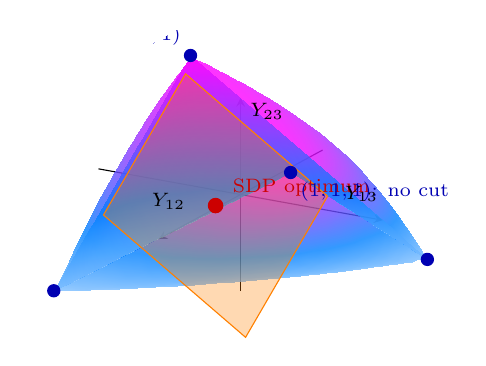
\begin{tikzpicture}
\begin{axis}[width=0.6\linewidth,height=0.48\linewidth,view={120}{28},axis lines=center,xlabel={$Y_{12}$},ylabel={$Y_{13}$},zlabel={$Y_{23}$},xmin=-1.2,xmax=1.2,ymin=-1.2,ymax=1.2,zmin=-1.2,zmax=1.2,ticks=none,xlabel style={font=\scriptsize},ylabel style={font=\scriptsize},zlabel style={font=\scriptsize}]
\addplot3[surf,shader=interp,opacity=0.8,colormap/cool,domain=-1:1,y domain=-1:1,samples=35,samples y=35,z buffer=sort] {x*y + sqrt(max(0,(1-x^2)*(1-y^2)))};
\addplot3[surf,shader=interp,opacity=0.8,colormap/cool,domain=-1:1,y domain=-1:1,samples=35,samples y=35,z buffer=sort] {x*y - sqrt(max(0,(1-x^2)*(1-y^2)))};
% objective hyperplane x+y+z = -1.5 (tangent at the SDP optimum), drawn as a patch
\addplot3[surf,fill opacity=0.3,color=orange,domain=-1.1:0.1,y domain=-1.1:0.1,samples=2,samples y=2,shader=flat,faceted color=orange!80!black] {-1.5 - x - y};
\addplot3[only marks,mark=*,mark size=2.2pt,color=blue!70!black] coordinates {(1,1,1) (1,-1,-1) (-1,1,-1) (-1,-1,1)};
\addplot3[only marks,mark=*,mark size=2.6pt,color=red!80!black] coordinates {(-0.5,-0.5,-0.5)};
\node[font=\scriptsize,red!80!black,anchor=south west] at (axis cs:-0.5,-0.5,-0.5) {\ SDP optimum};
\node[font=\scriptsize,blue!70!black,anchor=south east] at (axis cs:-1,-1,1) {cut $(-1,-1,1)$};
\node[font=\scriptsize,blue!70!black,anchor=north west] at (axis cs:1,1,1) {$(1,1,1)$: no cut};
\end{axis}
\end{tikzpicture}
\end{center}
\ona{\begin{figure}[htb]\caption{The spectrahedron of $3\times3$ correlation matrices (elliptope), with its four rank-one vertices, the cuts of a triangle, and the level set $Y_{12}+Y_{13}+Y_{23} = -\tfrac32$ of the MaxCut objective touching it at the SDP optimum, the three vectors at $120^\circ$. Level sets closer to the origin, e.g., $Y_{12}+Y_{13}+Y_{23} = -1$, cut through the set and contain the cut vertices $(-1,-1,1)$ and its permutations.}\label{fig:ch01:elliptope}\end{figure}}
\onp{\scriptsize Vertices $=$ cuts (rank one); the linear objective's level sets are hyperplanes; the optimum is where the last one touches the curved surface, at $120^\circ$ vectors: $2.25 > 2 = \mathrm{OPT}$.}
\end{frame}

\begin{frame}\ft{Step 4: random-hyperplane rounding}
\ona{Given optimal vectors $v_1^\star,\dots,v_n^\star$, we need a cut. \citet{Goemans1995} pick a uniformly random unit vector $r \in \R^n$ (e.g., $r = g/\|g\|$ with $g \sim \mathcal N(0, \one_n)$) and set}
\begin{equation}\label{eq:ch01:rounding}
    z_i = \sgn(r^\top v_i^\star), \qquad i \in V,
\end{equation}
\ona{i.e., the hyperplane through the origin with normal $r$ splits the sphere in two, and each vertex joins the side its vector lies on. Everything rests on one lemma.}
\begin{lem}[Probability of cutting an edge]\label{lem:ch01:arcs}
For unit vectors $v_i, v_j$ at angle $\theta_{ij} = \arccos(v_i^\top v_j) \in [0,\pi]$,
\begin{equation}
    \mathrm{Pr}\big[\sgn(r^\top v_i) \neq \sgn(r^\top v_j)\big] \;=\; \frac{\theta_{ij}}{\pi}.
\end{equation}
\end{lem}
\ona{\emph{Proof.} Let $P$ be the two-dimensional plane spanned by $v_i$ and $v_j$. Whether $r^\top v_i$ and $r^\top v_j$ have different signs depends only on the orthogonal projection $\bar r$ of $r$ onto $P$, and by rotational symmetry of the Gaussian, the direction of $\bar r$ is uniform on the circle in $P$. Within $P$, the line orthogonal to $\bar r$ separates $v_i$ from $v_j$ exactly when the direction of $\bar r$ falls into one of two arcs, each of angular length $\theta_{ij}$, namely the arc between the orthogonal complements of $v_i$ and $v_j$ and its antipodal copy. Total measure $2\theta_{ij}$ out of $2\pi$. \qed}
\onp{\emph{Proof.} Project $r$ onto the plane of $v_i, v_j$; its direction is uniform on the circle; it separates $v_i$ from $v_j$ iff it falls in one of two antipodal arcs of length $\theta_{ij}$: probability $2\theta_{ij}/2\pi$. \qed}
\end{frame}

\begin{frame}\ft{Random-hyperplane rounding, in pictures}
\begin{center}
\begin{tikzpicture}[scale=1.0,every node/.style={font=\scriptsize}]
% left: the two arcs argument
\begin{scope}
\draw[gray!60] (0,0) circle (1.3);
\draw[-{Stealth[length=4pt]},thick,blue!70!black] (0,0) -- (20:1.3) node[pos=1.15] {$v_i$};
\draw[-{Stealth[length=4pt]},thick,blue!70!black] (0,0) -- (85:1.3) node[pos=1.15] {$v_j$};
\draw[<->] (20:0.6) arc (20:85:0.6); \node at (52:0.85) {$\theta_{ij}$};
% arcs of directions of r that separate: perpendicular directions
\draw[red!70!black,very thick] (110:1.3) arc (110:175:1.3);
\draw[red!70!black,very thick] (290:1.3) arc (290:355:1.3);
\node[red!70!black] at (142:1.62) {length $\theta_{ij}$};
\node[red!70!black] at (322:1.62) {length $\theta_{ij}$};
% one sample hyperplane
\draw[dashed,thick,orange!90!black] (50:1.5) -- (230:1.5);
\draw[-{Stealth[length=4pt]},orange!90!black] (0,0) -- (140:0.9) node[pos=1.2] {$\bar r$};
\node at (0,-1.95) {$\mathrm{Pr}[\text{cut}] = \dfrac{2\theta_{ij}}{2\pi}$: $\bar r$ falls in a red arc};
\end{scope}
% right: pentagram cut by a random hyperplane
\begin{scope}[xshift=5.6cm]
\draw[gray!60] (0,0) circle (1.3);
\pgfmathsetmacro{\ang}{63}
\draw[dashed,thick,orange!90!black] ({\ang}:1.6) -- ({\ang+180}:1.6);
\draw[-{Stealth[length=4pt]},orange!90!black] (0,0) -- ({\ang+90}:0.8) node[pos=1.2] {$r$};
\foreach \i in {0,...,4}{
  \pgfmathsetmacro{\phi}{90+144*\i}
  \pgfmathsetmacro{\sgn}{cos(\phi-\ang-90)}
  \pgfmathparse{\sgn>0 ? "blue!70" : "orange!90!black"}\edef\col{\pgfmathresult}
  \draw[-{Stealth[length=4pt]},thick,\col] (0,0) -- ({\phi}:1.3) node[pos=1.18,\col] {$v_{\i}$};}
\node at (0,-1.95) {a random hyperplane splits the pentagram: here a $4$-edge cut};
\end{scope}
\end{tikzpicture}
\end{center}
\ona{\begin{figure}[htb]\caption{Left: the proof of Lemma~\ref{lem:ch01:arcs}. Project the random direction $r$ onto the plane of $v_i,v_j$; the hyperplane separates the two vectors exactly when the projected direction $\bar r$ lies in one of the two red arcs of angular length $\theta_{ij}$, so the probability is $2\theta_{ij}/2\pi$. Right: rounding the pentagram of Fig.~\ref{fig:ch01:c5}(b) with a random hyperplane; vectors on the same side receive the same colour. Adjacent vectors are $144^\circ$ apart, so each edge is cut with probability $144/180 = 0.8$, and the expected cut is $4 = \mathrm{OPT}$: on the 5-cycle the rounding loses nothing in expectation, although the relaxation overestimated.}\label{fig:ch01:rounding}\end{figure}}
\onp{\scriptsize On the 5-cycle each edge is cut with probability $144/180 = 0.8$, so $\mathbb E[W] = 4 = \mathrm{OPT}$, while $\mathrm{SDP} = 4.52$: the relaxation overestimates, the rounding recovers.}
\end{frame}

\begin{frame}\ft{Step 5: the performance ratio}
\ona{By linearity of expectation and Lemma~\ref{lem:ch01:arcs}, the expected weight of the rounded cut is}
\begin{equation}\label{eq:ch01:expcut}
    \mathbb E[W] = \sum_{(i,j)\in E} w_{ij}\,\frac{\theta_{ij}}{\pi},
    \qquad\text{while}\qquad
    \mathrm{SDP} = \sum_{(i,j)\in E} w_{ij}\,\frac{1-\cos\theta_{ij}}{2}.
\end{equation}
\ona{The two sums have the same weights and differ only in the function of $\theta_{ij}$ applied per edge. So compare the two functions \emph{per edge}, see Fig.~\ref{fig:ch01:gwratio}: define}
\begin{equation}\label{eq:ch01:alpha}
    \alpha_{\rm GW} \;\coloneqq\; \min_{0 < \theta \le \pi}\ \frac{\theta/\pi}{(1-\cos\theta)/2} \;=\; \min_{0<\theta\le\pi} \frac{2}{\pi}\,\frac{\theta}{1-\cos\theta} \;\approx\; 0.87856,
\end{equation}
\ona{attained at $\theta^\star \approx 2.33$ rad ($133.6^\circ$). Then $\theta_{ij}/\pi \ge \alpha_{\rm GW}(1-\cos\theta_{ij})/2$ for every edge, and since $w_{ij} \ge 0$,}
\begin{equation}
    \mathbb E[W] \;\ge\; \alpha_{\rm GW}\,\mathrm{SDP} \;\ge\; \alpha_{\rm GW}\,\mathrm{OPT}.
\end{equation}
\onp{Per edge, $\theta/\pi \ge \alpha_{\rm GW}\,(1-\cos\theta)/2$; sum with weights $w_{ij}\ge0$: $\ \mathbb E[W] \ge \alpha_{\rm GW}\,\mathrm{SDP} \ge \alpha_{\rm GW}\,\mathrm{OPT}$.}
\ona{That is the whole proof. Note that it bounds the cut against the relaxation value $\mathrm{SDP}$, which is computable, so the algorithm also certifies its own quality on every instance: $W/\mathrm{SDP}$ is a valid lower bound on $W/\mathrm{OPT}$.}
\end{frame}

\begin{frame}\ft{The two functions being compared}
\figslide[height=0.55\textheight]{figures/gw/gw_ratio.pdf}{Left: the per-edge contribution to the relaxation value, $(1-\cos\theta)/2$, and to the expected rounded cut, $\theta/\pi$, as functions of the angle $\theta$ between the two endpoint vectors. Right: their ratio, minimised at $\theta^\star \approx 2.33$ rad with value $\alpha_{\rm GW} \approx 0.8786$. Edges whose vectors are nearly antipodal ($\theta\approx\pi$) or nearly parallel ($\theta \approx 0$) lose nothing in the rounding; the loss is concentrated around $\theta^\star$.}{fig:ch01:gwratio}
\end{frame}

\begin{frame}\ft{Remarks on Goemans--Williamson}
\begin{itemize}\setlength\itemsep{0.3em}
    \item \textbf{Tightness.} The analysis is tight for the SDP: there are graphs with $\mathrm{OPT}/\mathrm{SDP} \to \alpha_{\rm GW}$, so no rounding of this relaxation can guarantee more. Under the Unique Games Conjecture, no polynomial-time algorithm at all, classical or quantum, beats $\alpha_{\rm GW}$ on all instances \cite{khot2010unique}; unconditionally, none beats $16/17 \approx 0.941$ unless $\mathbf P = \mathbf{NP}$ \cite{Hstad2001}.
    \item \textbf{Weights.} We used $w_{ij}\ge 0$ when summing the per-edge inequalities. With negative weights, i.e., general QUBO, the guarantee changes and the hardness factor becomes $11/13$ \cite{charikar2004maximizing}; \Chap~\chref{C.WSRounded}.
    \item \textbf{Randomness is removable} by the method of conditional expectations; in practice one simply draws many hyperplanes and keeps the best cut.
    \item \textbf{In practice} GW is much better than $0.878$: on the 144-node instances of \Chap~\chref{C.PerIteration}, ten hyperplanes find the optimum on all but a handful of instances, within ten seconds on a laptop.
    \item \textbf{Exercise.} Solve the SDP for the 5-cycle by hand (the pentagram) and compute $\mathrm{OPT}/\mathrm{SDP}$; you should get $\approx 0.8845$.
\end{itemize}
\end{frame}

\begin{frame}\ft{Where the quantum algorithm enters}
\ona{Hold on to two ideas from this section.}
\begin{itemize}\setlength\itemsep{0.4em}
    \item \textbf{Measurement is randomized rounding.} Measuring a product state $\bigotimes_i(\sqrt{1-c_i}\ket0 + \sqrt{c_i}\ket1)$ returns bit $i$ equal to $1$ with probability $c_i$, independently: this is the coordinate-wise randomized rounding of a fractional solution $c \in [0,1]^n$. QAOA replaces the product state by an entangled one, and the question is whether the entangling layers round \emph{better}.
    \item \textbf{A relaxation is a warm start.} The GW vectors, or the rounded GW cut, are the best polynomial-time information we have about the instance. Cold-start QAOA ignores it and starts from $\ket{+}^{\otimes n}$, i.e., from the uniformly random cut with ratio $1/2$. The rest of this lecture shows the consequences, and how warm starts repair them.
\end{itemize}
\end{frame}

\section{Hands-on: MaxCut three ways}\label{sec:ch01:code}

\begin{frame}\ft{One instance, three solvers}
\ona{Before the plots from the literature, let us solve one small instance ourselves, with the tools you will use in the assignments. The instance is a random 4-regular graph on 12 vertices with integer weights in $\{1,\dots,9\}$; it is generated, solved, and plotted by \texttt{code/ch01\_maxcut\_examples.py} in the course repository, which produces every number and figure in this section. Three solvers:}
\begin{enumerate}\setlength\itemsep{0.3em}
    \item \textbf{Exact}, with Gurobi via \texttt{gurobipy}: the integer quadratic program \eqref{eq:ch01:mcqp}. Branch and bound with cutting planes; exponential in the worst case, instantaneous here.
    \item \textbf{Relaxation and rounding}, with \texttt{cvxpy} and the SDP solver SCS: the semidefinite program \eqref{eq:ch01:sdp}, then Goemans--Williamson hyperplanes \eqref{eq:ch01:rounding}.
    \item \textbf{Variational}, with Qiskit: QAOA \eqref{eq:ch01:qaoa} simulated exactly on the statevector, angles optimised by COBYLA; from a cold start and from a warm start.
\end{enumerate}
\ona{Twelve qubits are simulable exactly, so we see the algorithms' behaviour without hardware noise.}
\end{frame}

\begin{frame}[fragile]\ft{Exact: Gurobi}
\begin{lstlisting}
import gurobipy as gp
m = gp.Model("maxcut")
x = m.addVars(n, vtype=gp.GRB.BINARY)          # x_i = 1 iff vertex i in S
# edge (i,j) is cut iff x_i != x_j, i.e. x_i + x_j - 2 x_i x_j = 1
m.setObjective(gp.quicksum(w * (x[i] + x[j] - 2 * x[i] * x[j])
                           for i, j, w in edges), gp.GRB.MAXIMIZE)
m.optimize()
z_opt = [1 - 2 * round(x[i].X) for i in range(n)]   # z_i in {-1,+1}
OPT = m.ObjVal                                       # 100 on our instance
\end{lstlisting}
\ona{Gurobi proves optimality: the maximum cut has value $\mathrm{OPT} = 100$, Fig.~\ref{fig:ch01:code1} (left). On twelve vertices this takes milliseconds; the same code scales to a few hundred vertices before the exponential worst case bites, and to thousands on sparse instances.}
\onp{Proves optimality: $\mathrm{OPT} = 100$ in milliseconds.}
\end{frame}

\begin{frame}[fragile]\ft{Relaxation: cvxpy and an SDP solver}
\begin{lstlisting}
import cvxpy as cp
Y = cp.Variable((n, n), symmetric=True)              # Gram matrix Y_ij = v_i . v_j
obj = 0.5 * sum(w * (1 - Y[i, j]) for i, j, w in edges)
sdp = cp.Problem(cp.Maximize(obj), [Y >> 0, cp.diag(Y) == 1])   # PSD, unit diagonal
sdp.solve(solver=cp.SCS, eps=1e-8)                   # SDP = 101.508 >= OPT
evals, evecs = np.linalg.eigh(Y.value)               # factor Y = V^T V ...
V = (evecs * np.sqrt(np.clip(evals, 0, None))).T     # ... columns v_i are unit vectors
def gw_round(V, rng):                                # random-hyperplane rounding
    r = rng.normal(size=n)                           # direction uniform on the sphere
    return np.sign(r @ V)                            # z_i = sgn(r . v_i)
\end{lstlisting}
\ona{The relaxation value is $\mathrm{SDP} = 101.51$, so $\mathrm{OPT}/\mathrm{SDP} = 0.985$: the relaxation is not exact on this instance, but it is far tighter than the worst case $\alpha_{\rm GW}$. The Gram matrix, Fig.~\ref{fig:ch01:code1} (right), already shows the cut: adjacent vertices have $Y_{ij}$ close to $-1$.}
\onp{$\mathrm{SDP} = 101.51$, $\mathrm{OPT}/\mathrm{SDP} = 0.985$.}
\end{frame}

\begin{frame}\ft{Exact solution and SDP solution}
\figslide[height=0.55\textheight]{figures/code/maxcut_gurobi_sdp.pdf}{Left: the instance with its maximum cut from Gurobi (dashed edges are cut, colours give the two sides, edge labels are weights). Right: the optimal SDP matrix $Y$ from cvxpy/SCS; entries near $-1$ mark vertex pairs the relaxation wants on opposite sides. Generated by \texttt{code/ch01\_maxcut\_examples.py}.}{fig:ch01:code1}
\end{frame}

\begin{frame}\ft{Rounding: what 1000 hyperplanes give}
\figslide[height=0.5\textheight]{figures/code/maxcut_gw_hist.pdf}{Distribution of the cut value over 1000 random hyperplanes, against the optimum (Gurobi), the relaxation value (cvxpy), the guarantee $\alpha_{\rm GW}\cdot\mathrm{SDP}$, and the empirical mean. Generated by \texttt{code/ch01\_maxcut\_examples.py}.}{fig:ch01:code2}
\ona{The mean rounded cut is $94.6$, i.e., $0.946\,\mathrm{OPT}$, comfortably above the guarantee $\alpha_{\rm GW}\,\mathrm{SDP} = 89.1$; a third of the hyperplanes hit the optimum, and the best of ten hyperplanes is optimal in $98\%$ of trials. This is what QAOA is competing against, on twelve vertices and at a cost of milliseconds.}
\onp{Mean $0.946\,\mathrm{OPT}$; guarantee $\alpha_{\rm GW}\mathrm{SDP} = 89.1$; best of ten hyperplanes optimal in $98\%$ of trials.}
\end{frame}

\begin{frame}[fragile]\ft{Variational: QAOA in Qiskit}
\begin{lstlisting}
from qiskit import QuantumCircuit
from qiskit.quantum_info import Statevector
def qaoa_circuit(betas, gammas, warm=None, eps=0.25):
    qc = QuantumCircuit(n)
    if warm is None: qc.h(range(n))                  # cold start |+>^n
    else:                                            # warm start from a cut z
        c = np.where(warm < 0, 1 - eps, eps)         # P(x_i = 1) = c_i
        thetas = 2 * np.arcsin(np.sqrt(c))
        for q in range(n): qc.ry(thetas[q], q)
    for beta, gamma in zip(betas, gammas):
        for i, j, w in edges: qc.rzz(gamma * w, i, j)            # exp(-i gamma H_C)
        for q in range(n):
            if warm is None: qc.rx(2 * beta, q)                  # exp(-i beta X)
            else:                                        # rotated mixer
                qc.ry(thetas[q], q); qc.rz(-2 * beta, q)
                qc.ry(-thetas[q], q)
    return qc
\end{lstlisting}
\ona{The cost unitary is one $ZZ$ rotation per edge and the mixer one $X$ rotation per qubit; the warm start replaces the Hadamards by $Y$ rotations encoding the cut and rotates the mixer accordingly, cf.\ \Chap~\chref{C.WSRounded}.}
\end{frame}

\begin{frame}[fragile]\ft{Variational: the classical optimizer}
\begin{lstlisting}
from scipy.optimize import minimize
def expected_cut(theta, p, warm=None):               # exact, from the statevector
    sv = Statevector(qaoa_circuit(theta[:p], theta[p:], warm)).data
    return float(np.abs(sv) ** 2 @ cut_of_basis)     # cut value of each basis state
res = minimize(lambda t: -expected_cut(t, p), theta0, method="COBYLA")
\end{lstlisting}
\ona{On hardware, \texttt{expected\_cut} would be replaced by sampling the circuit a few thousand times and averaging the cut values of the bitstrings; the statevector gives us the exact expectation and, for twelve qubits, the exact distribution of what sampling would return. The angles are optimised by COBYLA from several starting points: a grid scan at $p=1$ (the landscape in Fig.~\ref{fig:ch01:code3}), a linear ramp, the depth-$(p-1)$ optimum padded with a trivial layer, and random points.}
\onp{On hardware, replace the statevector by a few thousand shots. COBYLA from several starts: grid scan at $p=1$, linear ramp, padded depth-$(p-1)$ optimum, random.}
\end{frame}

\begin{frame}\ft{Variational: what QAOA gives on the same instance}
\figslide[height=0.5\textheight]{figures/code/maxcut_qaoa.pdf}{Left: the depth-one cold-start landscape $\langle\mathrm{cut}\rangle(\beta,\gamma)$, periodic and with several local maxima even in two dimensions. Right: cumulative distribution of the cut value of a sampled bitstring for the optimised states, against uniform sampling; the vertical lines mark the optimum and the GW cut used for the warm start. Generated by \texttt{code/ch01\_maxcut\_examples.py}.}{fig:ch01:code3}
\end{frame}

\begin{frame}\ft{Reading the numbers}
\begin{center}\ona{\small}\onp{\scriptsize}
\begin{tabular}{lrrr}\toprule
 & $\langle\mathrm{cut}\rangle/\mathrm{OPT}$ & $\mathrm{Pr}[\text{optimum}]$ & $\mathrm{Pr}[\text{cut} \ge 91]$ \\\midrule
uniform random cut & $0.60$ & $0.0005$ & $0.008$ \\
cold-start QAOA, $p=1$ & $0.796$ & $0.012$ & $0.13$ \\
cold-start QAOA, $p=2$ & $0.833$ & $0.025$ & $0.21$ \\
cold-start QAOA, $p=3$ & $0.854$ & $0.036$ & $0.27$ \\
warm-start QAOA (GW cut $91$), $p\le 3$ & $0.910$ & $0.000$ & $1.00$ \\
GW rounding, one hyperplane & $0.946$ & $0.35$ & $0.81$ \\
GW rounding, best of ten & $\approx 1$ & $0.98$ & $1.00$ \\
Gurobi & $1$ & $1$ & $1$ \\\bottomrule
\end{tabular}
\end{center}
\ona{Three observations. First, the cold start improves with depth but slowly: after three layers and some hundred COBYLA iterations per restart, the expected cut is $85\%$ of the optimum and the optimum is sampled $3.6\%$ of the time, below a single GW hyperplane. Second, the warm start does exactly what the analysis promised: at $\beta_1 = \pi/2$, $\gamma_1 = 0$ it reproduces its GW cut, and COBYLA finds nothing better at $p \le 3$ on this instance, so the guarantee is inherited and the circuit adds nothing here; the improvements beyond GW in Fig.~\ref{fig:ch01:eps} appear on larger, denser instances and with $\varepsilon$ tuned. Third, the whole variational pipeline costs minutes of statevector simulation, against milliseconds for the exact solver. Keep this table in mind when reading the utility-scale results next.}
\onp{Cold start: slow gains with depth, below one GW hyperplane. Warm start: inherits its GW cut exactly, no gain at $p\le3$ here. Cost: minutes versus milliseconds.}
\end{frame}

\section{The bad news: QAOA from a cold start}

\begin{frame}\ft{Bad news I: the angles are hard to find}
\ona{The landscape $F_p(\boldsymbol\theta)$ is a trigonometric polynomial in $2p$ variables, riddled with local minima even at $p=1$ \cite{Vijendran2025}. Worse, finding the global minimum is provably hard:}
\begin{itemize}\setlength\itemsep{0.3em}
    \item Training a VQA to additive error below $(1-\alpha_{\max})/2$ is \textbf{NP}-hard \cite{bittel2021training}, even for a single layer, and even on logarithmically many qubits.
    \item Deciding the depth $p$ needed to reach a target energy is \textbf{QCMA}-hard \cite{bittelQCMA}.
    \item In an idealised digitised setting, deciding whether a depth-58 QAOA reaches a target energy is \emph{undecidable} \cite{korpas2025undecidable}.
\end{itemize}
\ona{The proofs exhibit persistent local minima bounded away from the global optimum, in which gradient methods get trapped unless one restarts or injects noise \cite{kungurtsev2022iteration}. There are tractable regimes, e.g., a constant number of angles \cite{sakos2026global}, but they are the exception.}
\end{frame}

\begin{frame}\ft{Bad news II: even the best angles do not help at constant depth}
\ona{A complementary line of work shows that constant-depth QAOA fails on important instance families \emph{regardless of the angles}:}
\begin{itemize}\setlength\itemsep{0.3em}
    \item \textbf{Symmetry.} The state \eqref{eq:ch01:qaoa} inherits the $\mathbb{Z}_2$ spin-flip symmetry of $H_C$ and $H_M$, so $\langle Z_i\rangle = 0$ everywhere. On bipartite $D$-regular graphs, GW provably beats QAOA at any constant $p$ \cite{Bravyi2020}.
    \item \textbf{Locality.} A depth-$p$ circuit sees only the $p$-neighbourhood of each vertex; on high-girth graphs QAOA is a local algorithm and cannot break symmetry \cite{BravyiKlieschKoenigTang2022,BarakMarwaha2022}.
    \item \textbf{Overlap gap.} On sparse random graphs with the overlap-gap property, \emph{every} quantum circuit of depth $p < \varepsilon \log n$ falls short of the optimum with high probability \cite{ChouLoveSandhuShi2021,ChenHuangMarwaha2023}.
\end{itemize}
\ona{None of this is repaired by a better optimizer. It is, however, repaired by changing the algorithm: recursive QAOA \cite{Bravyi2020} and warm starts \cite{egger2021warm} both break the symmetry and the locality, and the latter is where we are heading today.}
\end{frame}

\begin{frame}\ft{Bad news III: what actually happens on hardware}
\ona{Theory bounds the worst case; let us look at typical instances. Figure~\ref{fig:ch01:hwconv} shows a closed-loop optimization of depth-four QAOA on 100 qubits on \emph{ibm\_boston}, from \Chap~\chref{C.PerIteration}. The optimizer (COBYLA) needs some 80 iterations and 1.6 million samples, i.e., minutes of QPU time and comparable classical post-processing, and the best sample among all of them achieves an approximation ratio of $91.5\%$. The distribution of the quantum samples is shifted to the right of uniform sampling, but only modestly.}
\figslide[height=0.58\textheight]{figures/numerics/figure2.pdf}{Closed-loop training of depth-four QAOA on 100 qubits on \emph{ibm\_boston} \cite{marecek2026angles}. (a) Energy of the best $5\%$ of samples per iteration. (b) QPU and CPU time versus the number of samples. (c) Cumulative distribution of the approximation ratio of the quantum samples (green) versus uniform sampling (red); the best sample achieves $91.5\%$.}{fig:ch01:hwconv}
\end{frame}

\begin{frame}\ft{Bad news IV: even noiseless simulation needs depth}
\ona{Noise is not the only culprit. Figure~\ref{fig:ch01:sv} shows exact statevector simulations on graphs with up to 22 nodes, again from \Chap~\chref{C.PerIteration}. With the best available angle-setting methods, the approximation ratio starts around $82$--$88\%$ at depth two and climbs to about $97\%$ only at depth ten. On Erd\H{o}s--R\'enyi graphs, angles transferred from regular graphs without re-optimization stagnate near $92\%$. Depth ten on 100 qubits is, today, well beyond what noisy hardware executes faithfully.}
\figslide[height=0.58\textheight]{figures/numerics/figure17.pdf}{Noiseless statevector results for MaxCut \cite{marecek2026angles}. (a) Approximation ratio versus QAOA depth for three graph families; (b),(c) density and average degree of the instances; (d)--(f) fixed angles with and without re-optimization, against the Interp.\ method, per family.}{fig:ch01:sv}
\end{frame}

\begin{frame}\ft{Bad news V: quality versus cost at utility scale}
\ona{Figure~\ref{fig:ch01:cost} puts quality and cost on one plot for ten 144-node heavy-hex MaxCut instances executed on \emph{ibm\_boston}. Every marker is an angle-setting strategy; the horizontal axis is the total wall-clock time spent finding the angles and sampling, the vertical axis is the approximation ratio of the hardware samples. The ratios range from $76\%$ to $85\%$, and the expensive iterative methods, costing $10^3$--$10^5$ seconds of classical training, buy at most a couple of percentage points over the cheapest look-up strategies.}
\figslide[height=0.4\textheight]{figures/numerics/figure10.pdf}{Hardware approximation ratio versus total duration for ten 144-node heavy-hex MaxCut instances on \emph{ibm\_boston}, at depth (a) $p=5$ and (b) $p=10$ \cite{marecek2026angles}. Each colour is an angle-setting method; squares use Pauli propagation and triangles matrix-product states to evaluate the energy during training.}{fig:ch01:cost}
\end{frame}

\begin{frame}\ft{Bad news VI: the Pareto frontier}
\ona{Taking the best strategy for every budget gives the Pareto frontier of Fig.~\ref{fig:ch01:pareto}. The frontier saturates at an approximation ratio of about $84\%$, reached after some $10^3$ seconds. Recall that GW reaches $100\%$ on almost all of these instances in under ten seconds.}
\figslide[height=0.5\textheight]{figures/numerics/figure11.pdf}{Pareto frontier of hardware approximation ratio against total duration across angle-setting strategies, 144-node heavy-hex MaxCut on \emph{ibm\_boston} \cite{marecek2026angles}. Labels give the QAOA depth at which each strategy enters the frontier.}{fig:ch01:pareto}
\onp{GW: $100\%$ on almost all instances, in $<10$ s.}
\end{frame}

\begin{frame}\ft{Taking stock}
\onp{Cold-start QAOA, i.e., from $\ket{+}^{\otimes n}$ with the transverse-field mixer:}
\ona{Let us take stock of QAOA \emph{from a cold start}, i.e., from the symmetric initial state $\ket{+}^{\otimes n}$ with the transverse-field mixer:}
\begin{itemize}\setlength\itemsep{0.3em}
    \item the angles are \textbf{NP}-hard to find, and the landscape has many local minima;
    \item at constant depth, GW provably wins on natural instance families, whatever the angles;
    \item on hardware at utility scale, approximation ratios of $80$--$85\%$ after minutes to days of computation, versus GW's near-optimal cuts in seconds;
    \item and even without noise, depth ten is needed to approach $97\%$.
\end{itemize}
\ona{This is not an argument against variational methods. It is an argument against ignoring what is known classically: the symmetric initial state throws away the best polynomial-time solution we have, and the circuit then spends its depth rediscovering it.}
\onp{\medskip The cold start throws away the best classical solution we have.}
\end{frame}

\section{The good news: warm starts}

\begin{frame}\ft{Warm-starting quantum optimization}
\ona{The idea of \citet{egger2021warm} is borrowed from classical optimization, where solvers are routinely warm-started from a solution of a relaxation. For a QUBO $\min_{x\in\{0,1\}^n} x^\top\Sigma x + \mu^\top x$ with $\Sigma \succeq 0$, let $c^\star \in [0,1]^n$ solve the convex relaxation over $[0,1]^n$. Then:}
\begin{enumerate}\setlength\itemsep{0.3em}
    \item replace the initial state $\ket{+}^{\otimes n}$ by the product state
    \begin{equation}\label{eq:ch01:wsinit}
        \ket{\phi^\star} = \bigotimes_{i=1}^n R_Y(\theta_i)\ket{0}, \qquad \theta_i = 2\arcsin\sqrt{c_i^\star},
    \end{equation}
    so that measuring qubit $i$ yields $1$ with probability $c_i^\star$: the measurement is a randomized rounding of $c^\star$;
    \item replace the mixer $-\sum_i X_i$ by $H_M^{(\rm ws)} = \sum_i \big(-\sin\theta_i\, X_i - \cos\theta_i\, Z_i\big)$, whose ground state is $\ket{\phi^\star}$, so that the adiabatic argument for convergence still applies;
    \item for MaxCut, warm-start from a GW cut (a rounded SDP solution) instead, with a mixer chosen so that $\beta_1=\pi/2,\gamma_1=0$ reproduces the GW cut exactly.
\end{enumerate}
\ona{The third variant inherits the $\alpha_{\rm GW}$ guarantee for \emph{any} angles, and any optimization can only improve on it. Details are in \Chap~\chref{C.WSRounded}.}
\end{frame}

\begin{frame}\ft{Good news I: sampling the optimum}
\ona{Figure~\ref{fig:ch01:pevo} compares standard and warm-started QAOA on a six-asset portfolio-optimization instance with a budget constraint, encoded as a QUBO. The probability of sampling the optimal portfolio from the optimized trial state is more than five times higher with the warm start at every depth $p \le 5$, and the energy of the warm-started state reaches the ground energy $E_0$ already at depth two. Standard QAOA reaches $E_0$ at depth three but still fails to produce the optimum with high probability: the low energy comes from satisfying the budget penalty, not from finding the best portfolio. Keeping the warm initial state but the standard mixer (blue) is worse than either, which justifies changing the mixer.}
\figslide[height=0.58\textheight]{figures/warmstart/figure04.pdf}{(a) Probability of sampling the optimal portfolio and (b) energy of the optimized trial state versus depth $p$, for standard QAOA (orange), warm-start QAOA (green), and warm initial state with the standard mixer (blue); medians and quartiles over ten random initial angles \cite{egger2021warm}.}{fig:ch01:pevo}
\end{frame}

\begin{frame}\ft{Good news II: 250 instances at depth one}
\ona{Depth one is where near-term hardware lives. Figure~\ref{fig:ch01:depth1} solves 250 random portfolio instances at $p=1$. The cold-start energies pile up at $0.74\,E_0$: the depth-one variational form cannot do better than a fixed fraction of the ground energy from the symmetric initial state. The warm-start energies spread from $0.72$ to $1.0\,E_0$, with a large mass at the optimum. Panel (b) shows that the improvement is largest when the relaxed and the binary optimum overlap.}
\figslide[height=0.58\textheight]{figures/warmstart/figure05.pdf}{Depth-one QAOA on 250 random portfolio instances \cite{egger2021warm}. (a) Histogram of the optimized energy relative to $E_0$ with (orange) and without (blue) warm start. (b) Remaining gap of the warm start relative to that of the cold start, against the overlap of the relaxed and the binary optimum.}{fig:ch01:depth1}
\end{frame}

\begin{frame}\ft{Good news III: MaxCut and the GW warm start}
\ona{For MaxCut the relaxation is the GW semidefinite program, and one warm-starts recursive QAOA (RQAOA) from its rounded cuts. Figure~\ref{fig:ch01:maxcut} compares, on 100 random graphs of each of four types, the best of ten GW cuts (blue), standard RQAOA (orange), warm-start RQAOA (red), and a purely classical recursion on the GW correlations (black). Warm-start RQAOA finds the maximum cut in more instances than any alternative, most markedly on the hardest family, fully connected 30-node graphs with random weights, where it finds the optimum in 85 of 100 graphs against 29 for standard RQAOA.}
\figslide[height=0.5\textheight]{figures/warmstart/figure08.pdf}{Cut sizes relative to the maximum cut on 100 graphs per panel \cite{egger2021warm}: random graphs with edge probability $1/2$ and weights $\pm1$ with (a) 20 and (b) 30 nodes; fully connected graphs with weights in $\{-10,\dots,10\}$ with (c) 20 and (d) 30 nodes. Grey side panels count the maximum cuts found. Dashed line: hardness factor $11/13$.}{fig:ch01:maxcut}
\end{frame}

\begin{frame}\ft{Good news IV: beyond GW at depth one}
\ona{Warm-start QAOA interpolates between the GW cut and standard QAOA through a regularisation parameter $\varepsilon \in [0, 0.5]$ that bounds the rotation angles \eqref{eq:ch01:wsinit} away from $0$ and $\pi$; at $\varepsilon = 0.5$ one recovers $\ket{+}^{\otimes n}$. Figure~\ref{fig:ch01:eps} sweeps $\varepsilon$ for depth-one warm-start QAOA on ten fully connected 30-node graphs. At $\varepsilon=0$ the energy is that of the GW cut, $0.907$ of the maximum cut; at $\varepsilon = 0.25$ it rises to $0.929$, \emph{above} the GW cut it started from; and towards $\varepsilon = 0.5$, the cold start, it collapses.}
\figslide[height=0.58\textheight]{figures/warmstart/figure07.png}{Energy of depth-one warm-start QAOA relative to the maximum cut, as a function of the regularisation $\varepsilon$, for ten fully connected 30-node graphs each warm-started from five GW cuts \cite{egger2021warm}. Medians, quartiles, and individual runs; the dotted line marks the median at $\varepsilon=0.25$.}{fig:ch01:eps}
\end{frame}

\begin{frame}\ft{Good news V: and it still improves with depth}
\ona{Finally, the warm start does not freeze the algorithm at the classical solution. Figure~\ref{fig:ch01:depthmc} follows a six-node instance, warm-started from a suboptimal cut of size 23 where the maximum is 27: the probability of sampling the maximum cut grows and the energy falls with the depth $p$, as it must, since the depth-$(p+1)$ circuit contains the depth-$p$ one.}
\figslide[height=0.6\textheight]{figures/warmstart/figure10.pdf}{Warm-start QAOA on a six-node graph, initialised from a cut of size 23 (maximum 27) \cite{egger2021warm}: (a) probability of sampling the maximum cut and (b) energy versus depth, 30 random initial angles per depth.}{fig:ch01:depthmc}
\end{frame}

\begin{frame}\ft{Taking stock, again}
\begin{itemize}\setlength\itemsep{0.4em}
    \item A warm start costs one classical relaxation, i.e., seconds, and gives the quantum algorithm the classical guarantee for free: any angles, including $\boldsymbol\theta = 0$, are at least as good as GW.
    \item It breaks the $\mathbb{Z}_2$ symmetry and the locality barrier, so the constant-depth obstructions of the cold start no longer apply.
    \item Empirically, at the depths hardware can execute, it is the difference between sampling the optimum with probability $0.05$ and $0.75$.
\end{itemize}
\ona{The rest of the course explains the machinery behind these plots: why alternating layers converge at all (\Chaps~\chref{C.Annealing}--\chref{C.QAOA}), how many noisy evaluations the optimizer needs (\Chap~\chref{C.IterationComplexity}), how to set angles when the circuit cannot be simulated (\Chap~\chref{C.PerIteration}), and how relaxations, roundings, and mixers fit together (\Chap~\chref{C.WSRounded}).}
\end{frame}

\begin{frame}\ft{Outline of the remaining lectures}
\onp{\footnotesize}
\begin{enumerate}\setlength\itemsep{0.05em}\setcounter{enumi}{1}
    \item Is there an exponential quantum advantage for ground states? The evidence, and why the overlap $\eta$ is the crux.
    \item What no polynomial-time algorithm can do: $16/17$, $11/13$, the UGC, and the \textbf{NP}-hardness of training.
    \item The adiabatic theorem; annealing through an exponentially small gap on glued trees.
    \item VQE: ansätze, measurement, barren plateaus, and VQE as state preparation for early fault-tolerant algorithms.
    \item QAOA: MaxCut encoding, depth one, and an elementary convergence proof via Perron--Frobenius.
    \item Gradients from shifted circuits: the parameter-shift rule and its relatives.
    \item How many iterations with biased evaluations: SPSA, two-point, and PSR compared.
    \item What one iteration costs: shots, circuits, simulators, latency; angle setting on 144 qubits.
    \item Warm starts from a GW cut: inherited guarantees and recursive QAOA.
    \item Warm starts from a continuous relaxation: the rotated mixer and $\varepsilon$.
    \item Linear systems: VQLS and the early-fault-tolerant alternative.
    \item Portfolios: Markowitz, its QUBO encoding, and what warm-started QAOA delivers.
\end{enumerate}
\end{frame}

\begin{frame}[allowframebreaks]\ft{References}
\biblio
\end{frame}

\end{document}
